\iffalse
\documentclass[journal,12pt,twocolumn]{article}
\usepackage{graphicx}
\usepackage[none]{hyphenat}
\usepackage[margin=0.5in]{geometry}
\usepackage[cmex10]{amsmath}
\usepackage{array}
\usepackage{booktabs}
\usepackage{gensymb}
\usepackage{textcomp}
\title{\textbf{Line Assignment}}
\author{Manideep Parusha - FWC22004}
\date{\today}

\providecommand{\norm}[1]{\left\lVert#1\right\rVert}
\providecommand{\abs}[1]{\left\vert#1\right\vert}
\let\vec\mathbf
\newcommand{\myvec}[1]{\ensuremath{\begin{pmatrix}#1\end{pmatrix}}}
\newcommand{\mydet}[1]{\ensuremath{\begin{vmatrix}#1\end{vmatrix}}}
\providecommand{\brak}[1]{\ensuremath{\left(#1\right)}}

\begin{document}

\maketitle
\section*{Problem}
\fi
Show that the diagonals of a square are equal and bisect each other at right angles.
\solution This is obvious from Problems
\eqref{chapters/9/8/1/2}
and
\eqref{chapters/9/8/1/3}.

\iffalse
\section*{Solution}

\begin{figure}[H]
\centering
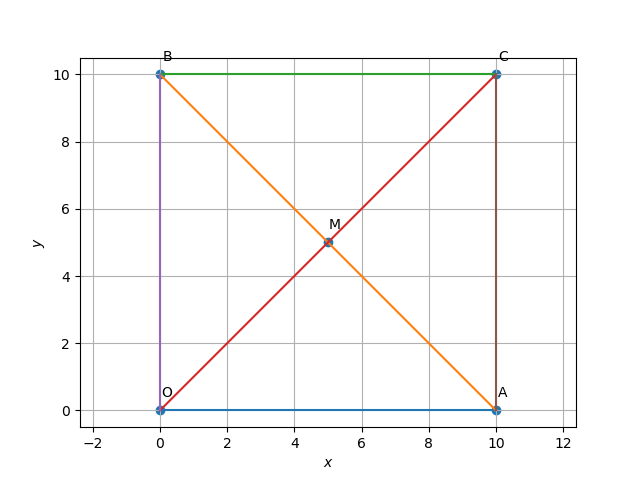
\includegraphics[width=0.75\columnwidth]{figs/sq_plot.png}
\caption{Square generated using python}
\label{fig:sq_py}
\end{figure}

\subsection*{Construction}
Inputs taken for the construction of the Square is 'a' , which is the side length of the square.
\begin{table}[H]
	\centering
\setlength\extrarowheight{2pt}
	\begin{tabular}{|c|c|c|}
		\hline
		\textbf{Symbol} & \textbf{Value} & \textbf{Description} \\
		\hline
		a & 10 & length of OA\\
		\hline
		O & (0,0) & point O\\
		\hline
		A & (a,0) & point A\\
		\hline
		B & (0,a) & point B\\
		\hline
		C & A+B & point C\\
		\hline
		M & $\frac{C}{2}$ & point M\\
		\hline
	\end{tabular}
\end{table}


Let OABC is a Square. Length of all sides are equal for a square and all interior angles equal to 90\degree.
O at the origin and vectors A, B \& C represent other vertices of the square.
\begin{align}
	\norm{\boldsymbol{OA}} = \norm{\boldsymbol{OB}} = \norm{\boldsymbol{BC}} = \norm{\boldsymbol{AC}} \\
\angle OAC = \angle OBC = \angle BCA = \angle AOB = 90\degree
\label{eq-1}
\end{align}
Here, $D_1$ and $D_2$ are the diagonals of the square and we can compute $D_1$ and $D_2$ as
\begin{equation}
	\boldsymbol{D_1 = (A + B) } \\
	\label{D1eq}
\end{equation}
\begin{equation}
	\boldsymbol{D_2 = (A - B) }
	\label{D2eq}
\end{equation}

To prove that the diagonals of the square are equal, we can find the length of the two diagonals and compare. Hence,
\begin{equation}
\norm {\boldsymbol{D_1}}  = \norm {\boldsymbol{A + B}}\\
	\label{D1_len}
\end{equation}
\begin{equation}
\norm {\boldsymbol{D_2}}  = \norm {\boldsymbol{A - B}}
	\label{D2_len}
\end{equation}
For finding length of $D_1$, we can write from equation \eqref{D1_len},  
\begin{align}
	\norm{\boldsymbol{A + B}} = \sqrt{\norm{\boldsymbol{A}}^2 + \norm{\boldsymbol{B}}^2 + 2\boldsymbol{A}^T\boldsymbol{B}}
	\label{extend_D1}
\end{align}
But, for a square we know that length of all sides are equal.
\begin{equation}
	\norm {\boldsymbol{A}} = \norm{\boldsymbol{B}}
	\label{equal_sides}
\end{equation}
and, the angle between two adjacent sides is 90\degree. The dot product of two vectors which are seperated by 90\degree angle is always '0'. 
\begin{equation}
	\boldsymbol{A}^T\boldsymbol{B} = 0 
	\label{dot_product_is_0}
\end{equation}
So the equation \eqref{extend_D1} becomes 
\begin{align}
	\norm {\boldsymbol{A + B}} = \sqrt{2}\norm{\boldsymbol{A}}\\
	\norm {\boldsymbol{D_1}} = \sqrt{2}\norm{\boldsymbol{A}} 
	\label{D1_length}
\end{align}
Similarly, for finding the length of $D_2$ 
\begin{align}
	\norm {\boldsymbol{A - B}} = \sqrt{\norm{\boldsymbol{A}}^2 + \norm{\boldsymbol{B}}^2 - 2\boldsymbol{A}^T\boldsymbol{B}}
\end{align}
But, from \eqref{equal_sides} and \eqref{dot_product_is_0}
\begin{align}
	\norm {\boldsymbol{A - B}} = \sqrt{2}\norm{\boldsymbol{A}}\\
	\norm {\boldsymbol{D_2}} = \sqrt{2}\norm{\boldsymbol{A}} 
	\label{D2_length}
\end{align}
So, from the equations \eqref{D1_length} and \eqref{D2_length}, we can say that the lengths of diagonals $\boldsymbol{D_1}$ and $\boldsymbol{D_2}$ are equal 
\begin{equation}
	\norm{\boldsymbol{D_1}} = \norm{\boldsymbol{D_2}}
\end{equation}





We know that, if the dot product of two vectors is zero then the vectors are perpendicular to each other. \\
So, by taking the dot product of $\boldsymbol{D_1}$ and $\boldsymbol{D_2}$ 
\begin{align}
	\boldsymbol{D_1.D_2} = \boldsymbol{D_1}^T \boldsymbol{D_2} \\
	\boldsymbol{D_1.D_2} = (\boldsymbol{A + B})^T(\boldsymbol{A - B})\\
	\boldsymbol{D_1.D_2} = \norm{\boldsymbol{A}}^2 - \norm{\boldsymbol{B}}^2
\end{align}	
From the equation \eqref{equal_sides}, 
\begin{align}
	\boldsymbol{D_1.D_2} = \norm{\boldsymbol{A}}^2 - \norm{\boldsymbol{A}}^2 \\
	\boldsymbol{D_1.D_2} = 0 
\end{align}	
as the dot product of the diagonals is equal to 0, we can say that both diagonals are perpendicular to each other. \\

Let diagonals $\boldsymbol{D_1}$ and $\boldsymbol{D_2}$ intersect at a point $\boldsymbol{M}$. We have to prove that $\boldsymbol{M}$ is the mid point of $\boldsymbol{D_1}$ and $\boldsymbol{D_2}$, in order to say that both diagonals bisect eachother.
\begin{align}
	\boldsymbol{OM} = x \boldsymbol{D_1}\\
	\boldsymbol{MA} = y \boldsymbol{D_2}
\end{align}
From the equations \eqref{D1eq} and \eqref{D2eq}, the above equations can be written as
\begin{align}
	\boldsymbol{OM} = x\boldsymbol{A + B}\\
	\boldsymbol{MA} = y\boldsymbol{A - B}
\end{align}
Now, if we consider
\begin{align}
	\boldsymbol{OA} = \boldsymbol{OM} + \boldsymbol{MA}\\
	\boldsymbol{A} = x(\boldsymbol{A+B}) + y(\boldsymbol{A-B})\\
	\boldsymbol{A} = x\boldsymbol{A} + x\boldsymbol{B} + y\boldsymbol{A} - y\boldsymbol{B}\\
	\boldsymbol{A} = (x+y)\boldsymbol{A} + (x-y)\boldsymbol{B}
\end{align}
Equating the co-efficient of $\boldsymbol{A}$ and $\boldsymbol{B}$, we get
\begin{align}
	x + y = 1 , x - y = 0\\
	2x = 1\\
	x = \frac{1}{2}\\
	y = \frac{1}{2}
\end{align}

now we can say that
\begin{align}
	\boldsymbol{OM} = \frac{1}{2} \boldsymbol{D_1}\\
	\boldsymbol{MA} = \frac{1}{2} \boldsymbol{D_2}
\end{align}
Hence, M is the mid point of diagonals $D_1$ and $D_2$ and we can say that both diagonals bisect eachother. \\

we have proved that diagonals of a square are equal in length and bisect eachother at right angles.





\end{document}
\fi
